\documentclass{jarticle}
\usepackage[dvipdfmx]{graphicx}
\usepackage{here}
\usepackage{listings,jlisting}


\lstset{
  basicstyle={\ttfamily},
  identifierstyle={\small},
  commentstyle={\smallitshape},
  keywordstyle={\small\bfseries},
  ndkeywordstyle={\small},
  stringstyle={\small\ttfamily},
  frame={tb},
  breaklines=true,
  columns=[l]{fullflexible},
  numbers=left,
  xrightmargin=0zw,
  xleftmargin=3zw,
  numberstyle={\scriptsize},
  stepnumber=1,
  numbersep=1zw,
  lineskip=-0.5ex
}

\title{{システム実験}\\基礎実験3}
\author{6119019056 山口力也}
\date{2019/05/10日提出}

\begin{document}
\maketitle
\section{電圧,ディジタル値との関係}
演習2.3.1の結果を報告し,その結果からAD変換結果(ディジタル値)と電圧のグラフを作成せよ.

\begin{itemize}

\item AD変換結果(ディジタル値)-$A_0$の計算上の電圧$V_o$[V]
\item AD変換結果(ディジタル値)-AD変換結果から求めた電圧[V]

\end{itemize}

以下図\ref{fig:enshu2-3-1riron},図\ref{fig:enshu2-3-1sokutei}に結果のグラフを示す.

\begin{figure}[H]
\begin{center}
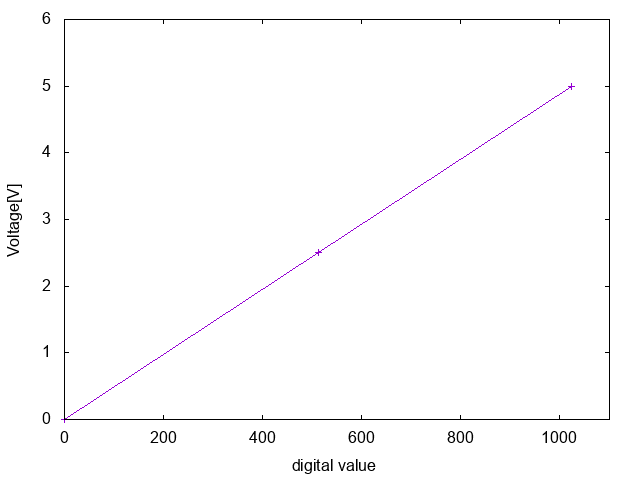
\includegraphics[width=7.0cm]{images/enshu2-3-1_riron.png}
\caption{演習2.3.1の結果(理論値)}
\label{fig:enshu2-3-1riron}
\end{center}
\end{figure}

\begin{figure}[H]
\begin{center}
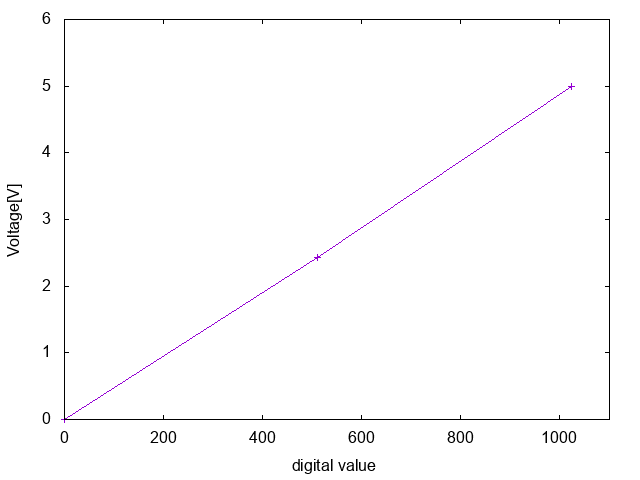
\includegraphics[width=7.0cm]{images/enshu2-3-1_sokutei.png}
\caption{演習2.3.1の結果(測定値)}
\label{fig:enshu2-3-1sokutei}
\end{center}
\end{figure}


\section{半固定抵抗によるLEDの点灯・消灯}
課題2.3.1において実装したブレッドボード配線図およびプログラムを報告せよ.シリアルモニタで確認した値とLEDの点灯・消灯の状況を報告せよ.さらにプログラム作成時に工夫した点を記せ.また,抵抗値を調整することで,なぜ図2.40の$A_0$の電圧が変化するのか,$A_0$における電圧を図2.38(b)を参考にして考察せよ.

以下図\ref{fig:kadai2-3-1bread}にブレッドボード配線図を示す.

\begin{figure}[H]
\begin{center}
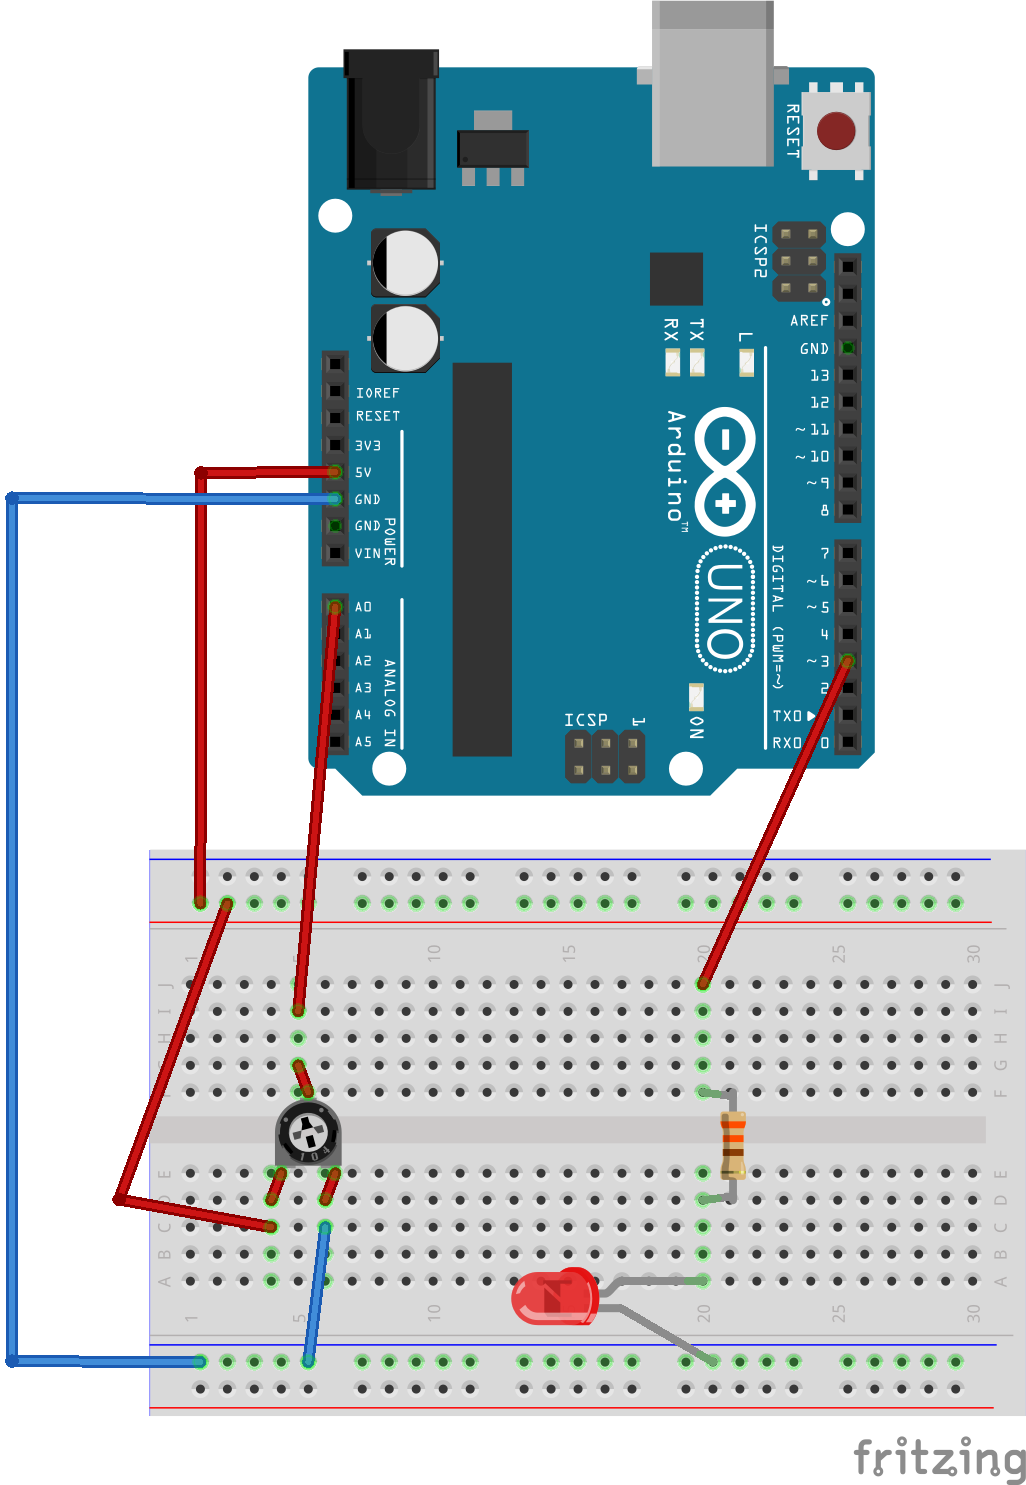
\includegraphics[width=7.0cm]{images/kadai2-3-1_bread.png}
\caption{課題2.3.1の配線図}
\label{fig:kadai2-3-1bread}
\end{center}
\end{figure}

以下ソースコード\ref{code:kadai2-3-1}にプログラムを示す.


\begin{lstlisting}[caption = 課題2.3.1,label=code:kadai2-3-1][H]
const int LED_PIN = 3;//LED_PINを定義
void setup() {
  Serial.begin(9600);
  // シリアル通信を9600kbpsで初期化
  pinMode(LED_PIN,OUTPUT);
  //LED_PINを出力に設定
}
void loop() {
  int sensorValue = analogRead(A0);//A0ピンのAD変換結果を取得する.
  float vo = sensorValue*(5.0/1024.0);//sensorValueの値を電圧値に変換
  Serial.println(vo);//システムモニタにvoを表示
  delay(1);        // 安定用
  if(vo>2.50){//2.5V以上なら
    digitalWrite(LED_PIN,HIGH);//LED点灯
  }
  else{//2.5V以下なら
    digitalWrite(LED_PIN,LOW);//LED消灯
  } 
}
\end{lstlisting}

シリアルモニタで確認した時

プログラム作成時に工夫した点は特にないが,LED\_PINを定義してわかりやすくした点である.閾値の2.50を定義して閾値の変更を容易にするともう少し良いプログラムになったと思う.
抵抗値を調整することで電圧が変化するのはオームの法則より,抵抗に流れる電流が変化し,電圧が変化するためである.

\section{照度センサによるLEDの点灯・消灯}

課題2.3.2において実装したブレッドボード配線図,プログラムおよびプログラムの実行結果を報告せよ.また,プログラム作成において工夫した点を記せ.演習2.3.3で作成したプログラムによる,シリアルモニタで確認した照度の最大値および最小値を報告せよ.作成したプログラムによる,明るさの変化とLEDの点灯・消灯の状況を報告せよ.

以下図\ref{fig:kadai2-3-2bread}にブレッドボード配線図を示す.

\begin{figure}[H]
\begin{center}
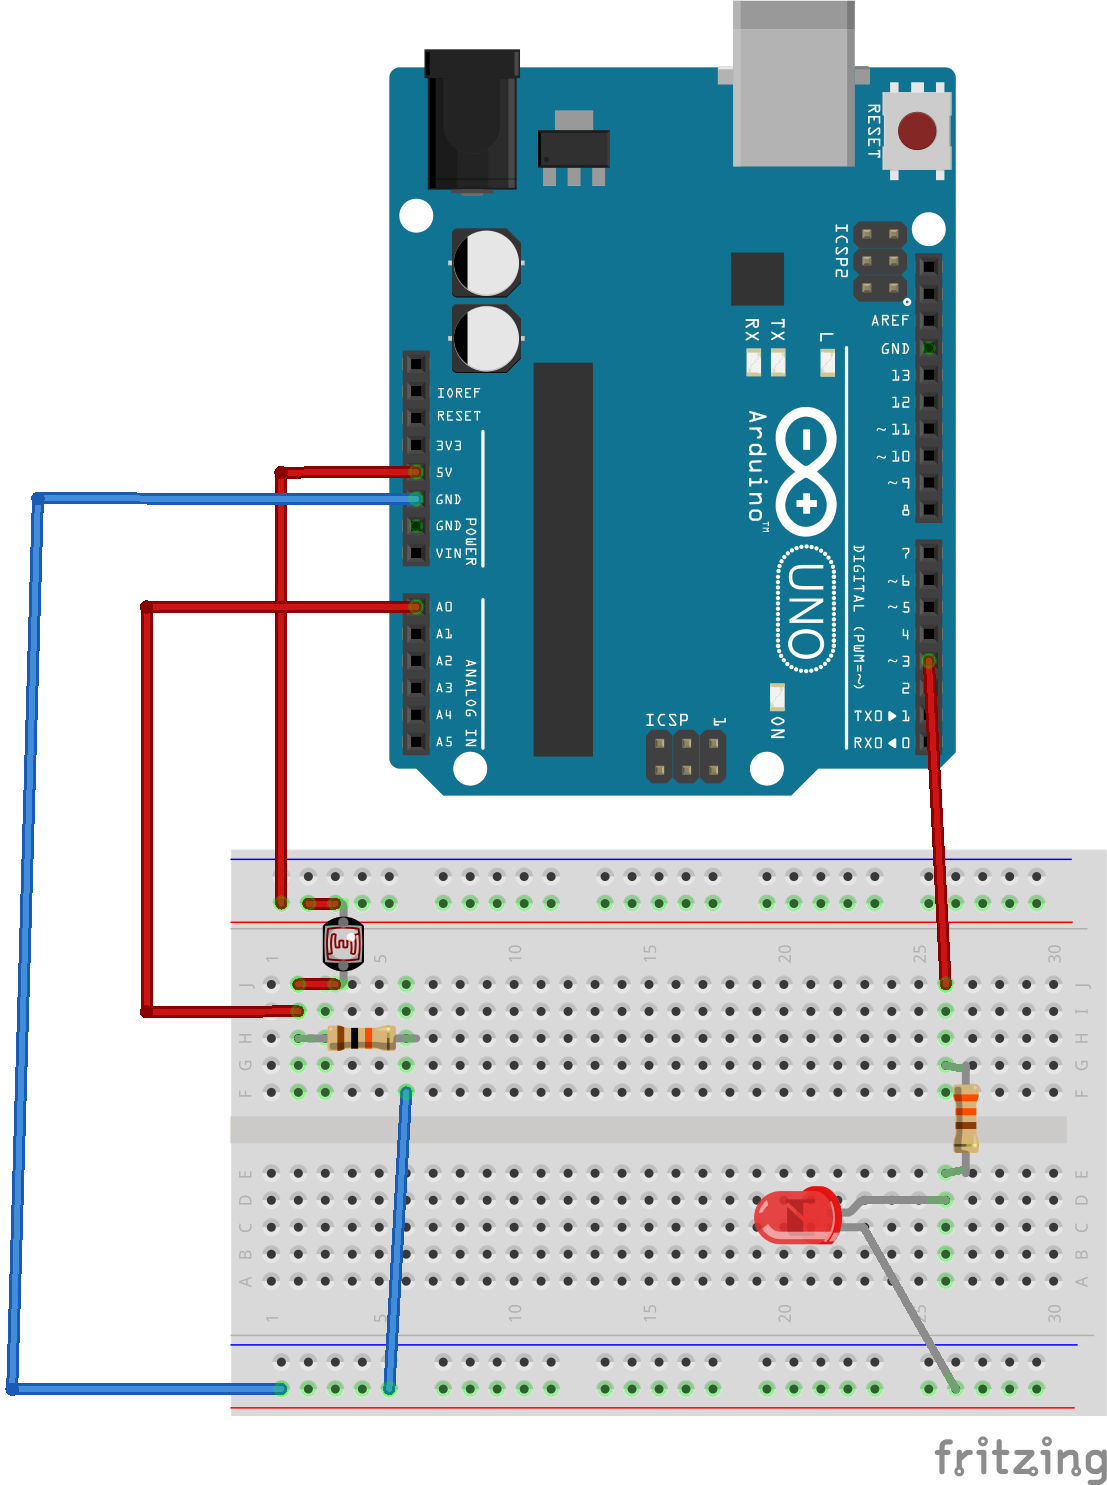
\includegraphics[width=7.0cm]{images/kadai2-3-2_bread.png}
\caption{課題2.3.2の配線図}
\label{fig:kadai2-3-2bread}
\end{center}
\end{figure}

また,以下ソースコード\ref{code:kadai2-3-2}にプログラムを示す.

\begin{lstlisting}[caption = 課題2.3.2,label=code:kadai2-3-2][H]
const int LED_PIN = 3; //LED_PINを3と定義
void setup() {
  Serial.begin(9600);
  // シリアル通信を9600kbpsで初期化
  pinMode(LED_PIN,OUTPUT);
  //LED_PINを出力に設定
}
void loop() {
  int sensorValue = analogRead(A0);//A0ピンのAD変換結果を取得する.
  float vo = sensorValue*(5.0/1024.0);//デジタル値を電圧値に変換
  float L =222*vo; //電圧を照度値に変換
  Serial.println(L); //照度値をシステムモニタに表示
  digitalWrite(LED_PIN,lux_threshold(L)); //LED_PINポートにthresholdの戻り値を出力
  delay(1);      //安定用 
}

int lux_threshold(float lux){ //中間値用
  int th_val = 0;
  if(lux > 1.08){//中間値(1.08)より大きいなら
    th_val = HIGH; //LED点灯
  }
  else{ //そうでないなら
    th_val = LOW; //LED消灯
  }
  return th_val; //th_valを返す
}
\end{lstlisting}

プログラムで工夫した点はデジタル値を電圧値,照度値に変換する時に一気にやるのではなく,一度電圧値に変換してから照度値に変換することでわかりやすく,また他のシステムでも使いやすくしたところである.ただ,$5.0/1024.0$や,関数lux\_thresholdの中間値の1.08なども定義すると状況が変わっても容易に変更できたと思う.
シリアルモニタで確認した照度値の最大値は2.17,最小値は0だった.LEDは明るい場合点灯し,暗い場合消灯した.

\section{ディジタルPWMによるLEDの明るさ調整}

演習2.3.4で実装したブレッドボード配線図,プログラムおよび演習結果(表)およびanalogWriteの引数と2つのLEDの明るさを見比べた結果を報告せよ.また,PWM制御によりなぜLEDの明るさが変化するのか,その理由を考察せよ.

以下図\ref{fig:enshu2-3-4bread}にブレッドボード配線図を示す.

\begin{figure}[H]
\begin{center}
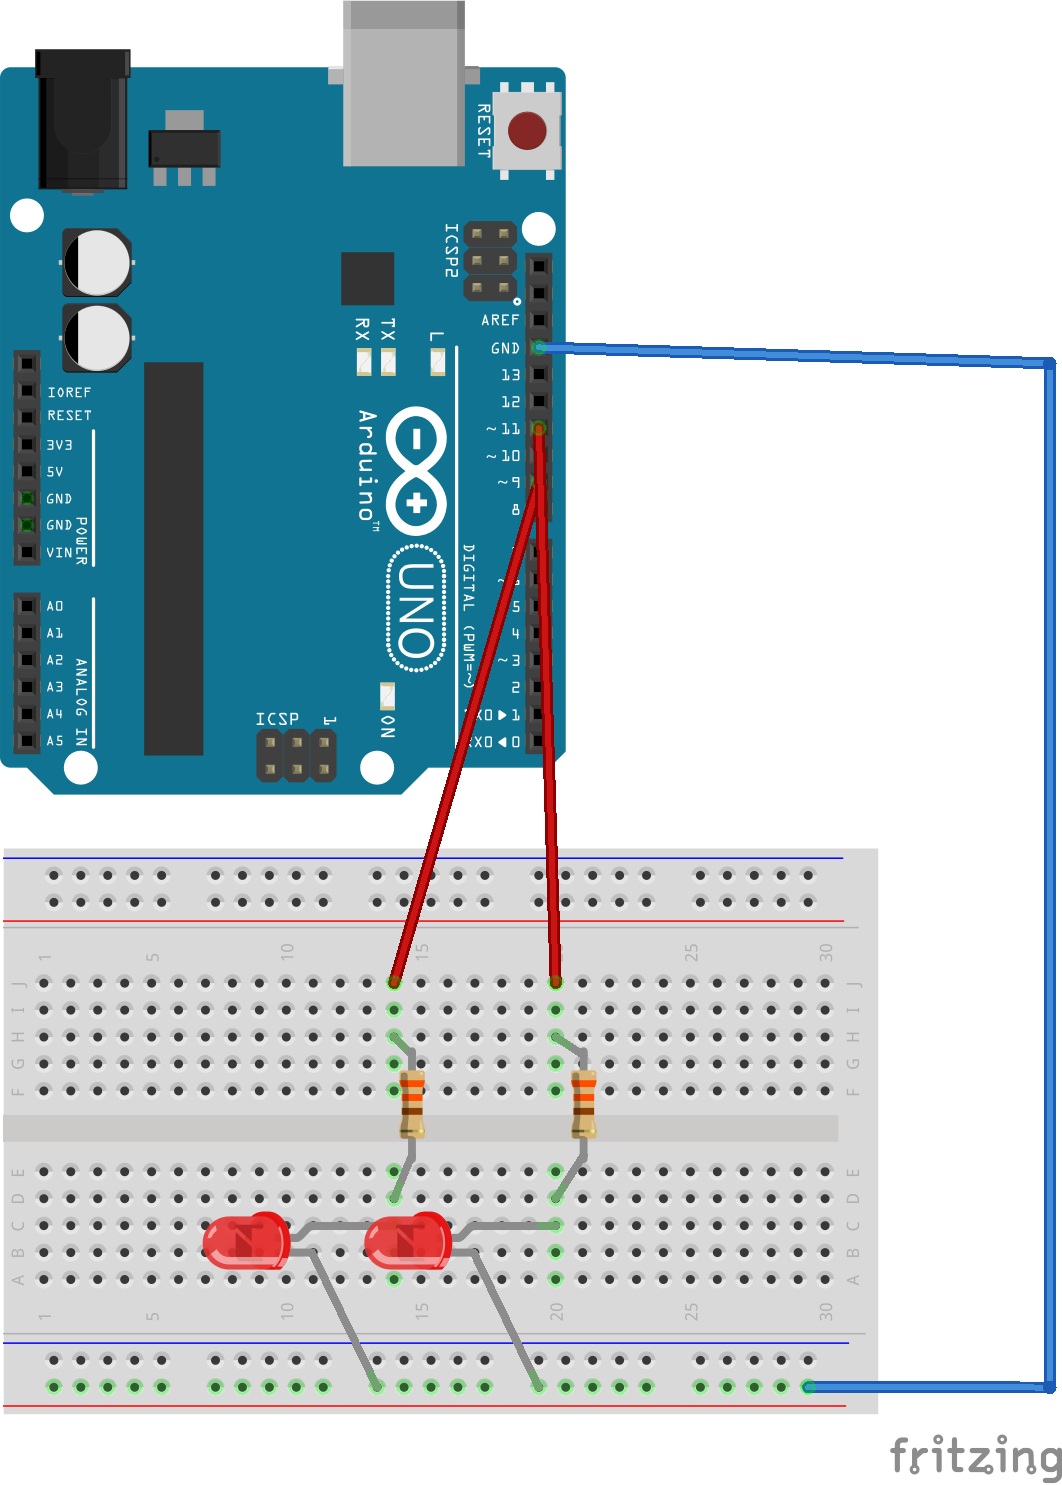
\includegraphics[width=7.0cm]{images/enshu2-3-4_bread.png}
\caption{演習2.3.4の配線図}
\label{fig:enshu2-3-4bread}
\end{center}
\end{figure}

また,以下ソースコード{code:enshu2-3-4}にプログラムを示す.

\begin{lstlisting}[caption = 演習2.3.4,label=code:enshu2-3-4][H]
//それぞれのポート番号を定義
const int LED_RED_PIN = 9; 
const int LED_YEL_PIN = 11;
void setup() {
  Serial.begin(9600);
  // シリアル通信を9600kbpsで初期化
  pinMode(LED_RED_PIN,OUTPUT);
  pinMode(LED_YEL_PIN,OUTPUT);
  //LEDのポートをそれぞれ出力に設定
}
void loop() {
    analogWrite(LED_RED_PIN,64);//赤色に25%出力
    analogWrite(LED_YEL_PIN,192);//黄色に75%出力
    delay(10);//安定用
  }
}
\end{lstlisting}

analogWriteの引数を大きくするとLEDの明るさは明るくなる.PWM制御によりLEDの明るさが変化するのは,デューティ比により見かけの電圧が変化するためである.電圧が変化するとLEDに流れる電流が変化するのでLEDの明るさも変化する.
以下表\ref{table:enshu2-3-4}に結果の表を示す.

\begin{table}[H]
\centering
\caption{演習2.3.4の結果}
\label{table:enshu2-3-4}
\begin{center}
\begin{tabular}{c|c}
\hline \hline
デューティ比[\%] & analogWriteの引数\\ \hline
0 & 0  \\
25 & 64 \\
50 & 128 \\
75 & 192 \\ 
100 & 255 \\ \hline
\end{tabular}
\end{center}
\end{table}

\section{ディジタルPWMによるLEDの明るさ調整2}

課題2.3.3で実装した,ブレッドボード配線図,プログラムおよび実験結果を報告せよ.また,プログラムで工夫した点を記せ.


以下図\ref{fig:kadai2-3-3bread}にブレッドボード配線図を示す.

\begin{figure}[H]
\begin{center}
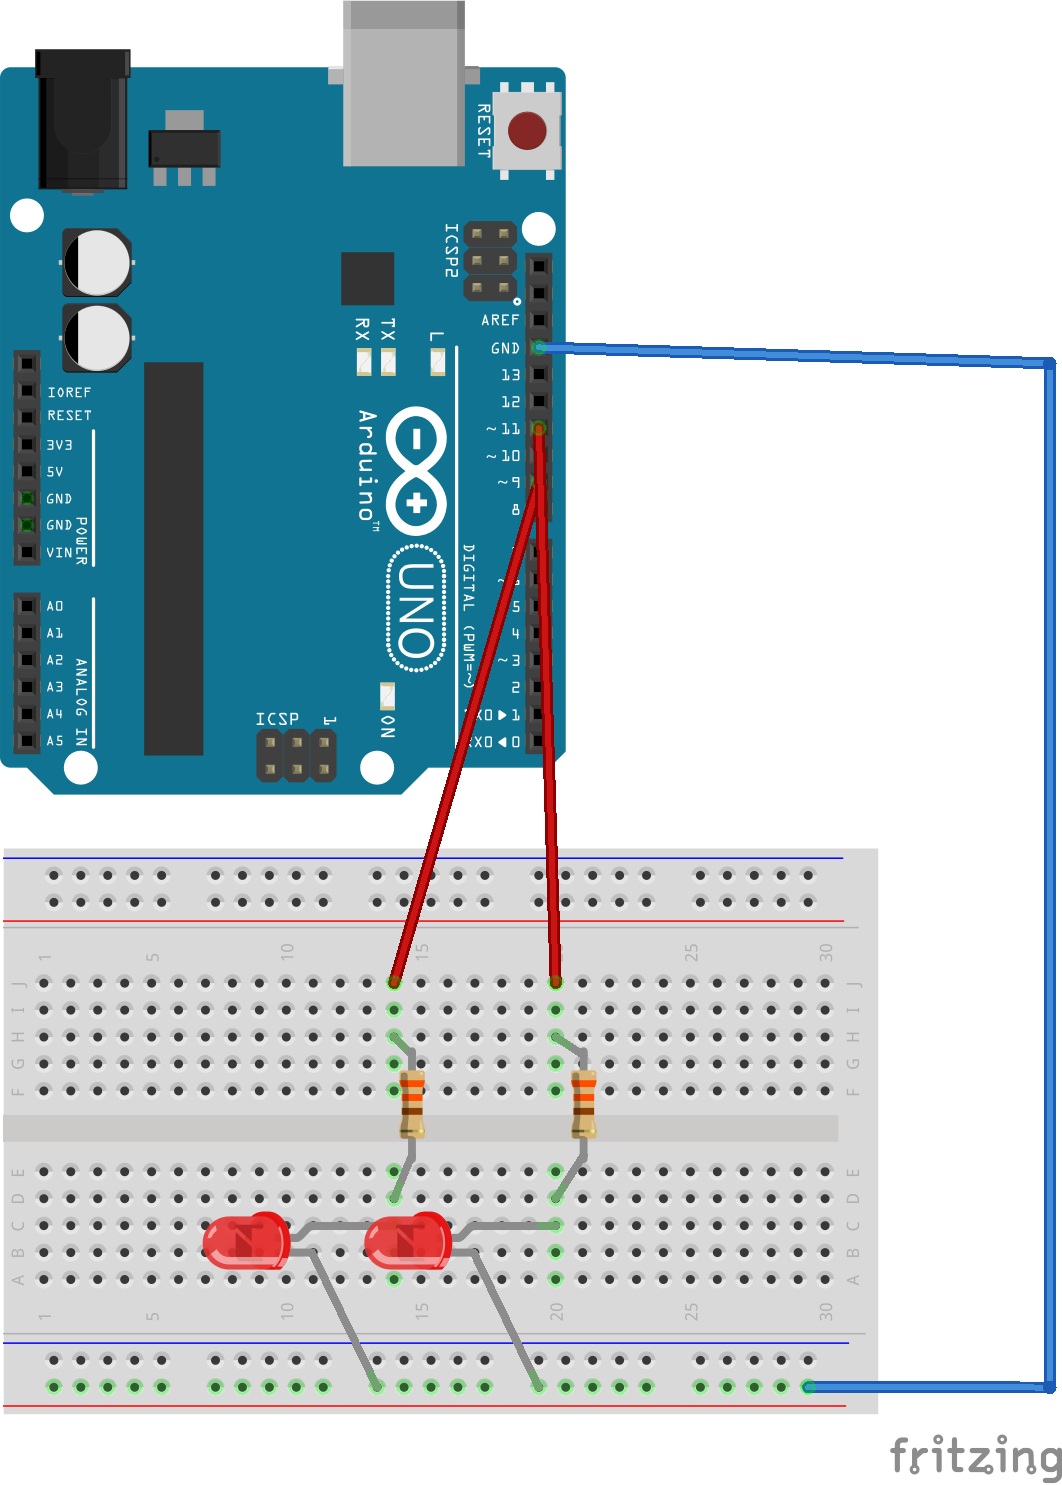
\includegraphics[width=7.0cm]{images/enshu2-3-4_bread.png}
\caption{課題2.3.3の配線図}
\label{fig:kadai2-3-3bread}
\end{center}
\end{figure}

また,以下ソースコード\ref{code:kadai2-3-3}にプログラムを示す.

\begin{lstlisting}[caption = 課題2.3.3,label=code:kadai2-3-3][H]
//それぞれのポート番号を定義
const int LED_RED_PIN = 9;
const int LED_YEL_PIN = 11;
void setup() {
  Serial.begin(9600);
  // シリアル通信を9600kbpsで初期化
  pinMode(LED_RED_PIN,OUTPUT);
  pinMode(LED_YEL_PIN,OUTPUT);
  //LEDのポートをそれぞれ出力に設定
}
void loop() {
  for(int i = 0; i <= 256; i+=64){
    if(i==256){//256は引数にならないので
      i--;
    }
    analogWrite(LED_RED_PIN,i);//それぞれにiを出力
    analogWrite(LED_YEL_PIN,i);//それぞれにiを出力
    delay(1000);//1秒待つ
  }
}
\end{lstlisting}

実験結果としては1秒ごとにLEDの明るさが変化した.プログラムで工夫した点はfor文の中でanalogWriteは256を引数に取らないのでif文をつけて条件化して256を排除したところである.

\section{発展課題2.3.1}

発展課題2.3.1で実装したブレッドボード配線図,プログラムおよび実験結果を報告せよ.また,圧電ブザーが鳴る原理について調査せよ.

以下図\ref{fig:hattenkadai2-3-1bread}にブレッドボード配線図を示す.

\begin{figure}[H]
\begin{center}
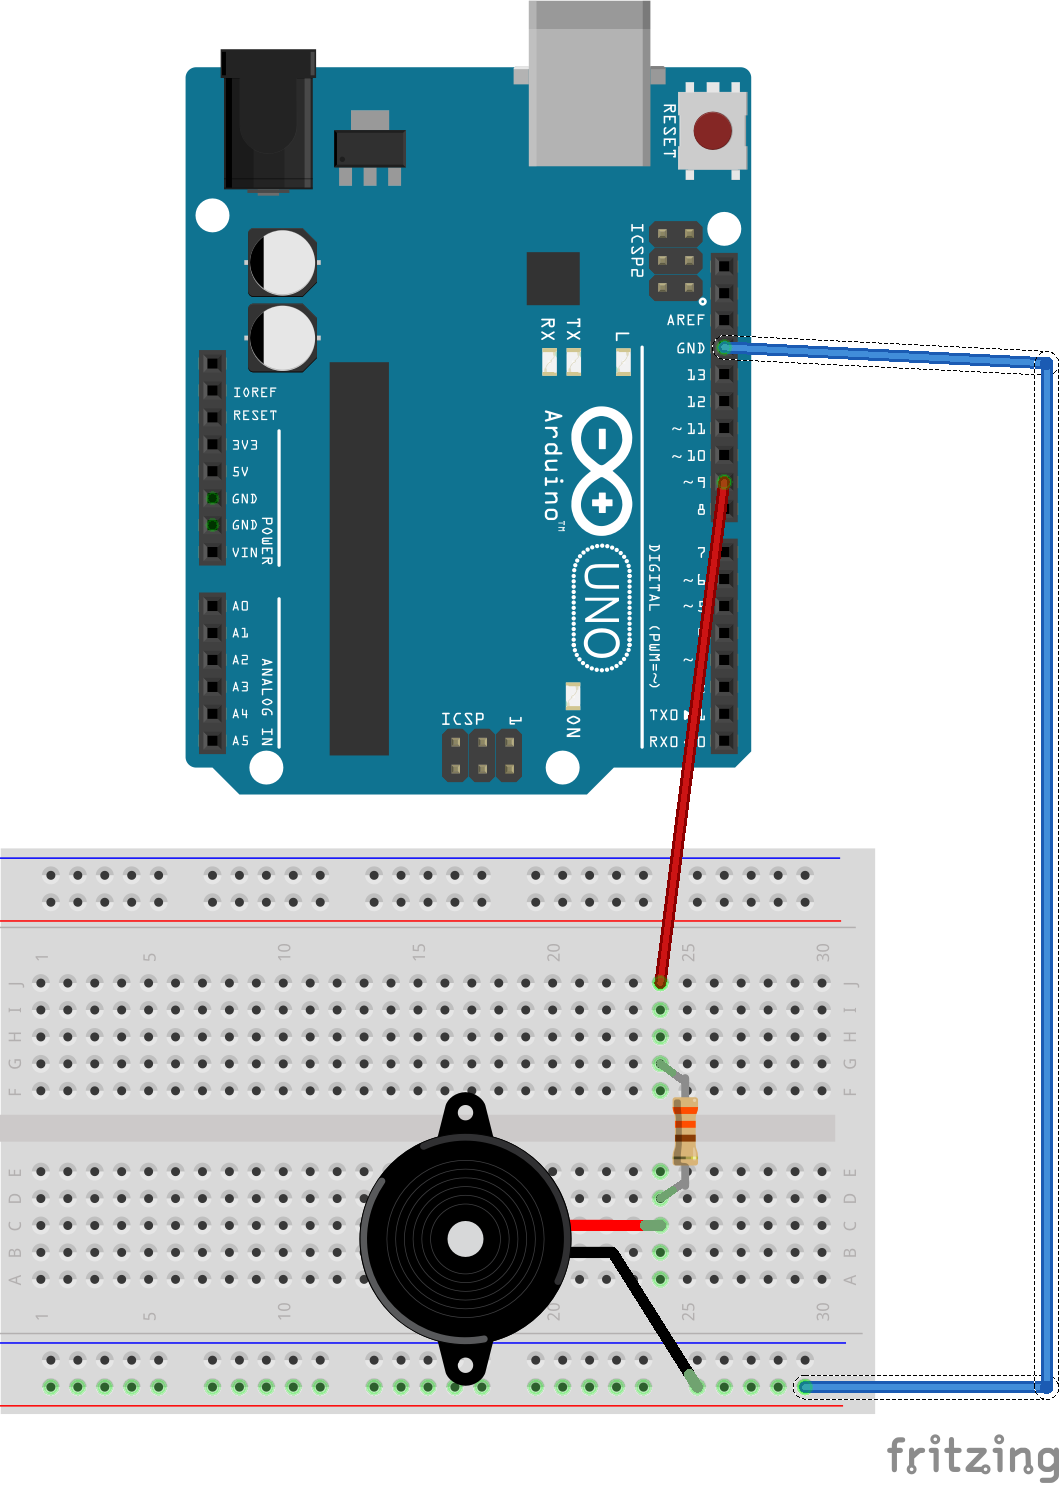
\includegraphics[width=7.0cm]{images/hatten2-3-1_bread.png}
\caption{発展課題2.3.1の配線図}
\label{fig:hattenkadai2-3-1bread}
\end{center}
\end{figure}

また,以下ソースコード\ref{code:hattenkadai2-3-1}にプログラムを示す.

\begin{lstlisting}[caption=発展課題2.3.1,label=code:hattenkadai2-3-1][H]
//値を定義
const int buzzer = 9;
void setup() {
  Serial.begin(9600);
  // シリアル通信を9600kbpsで初期化
  pinMode(buzzer,OUTPUT);
  //buzzerを出力に設定
}
void loop() {
  for(int i = 0; i <= 256; i+=64){
    if(i==256){//256は引数にならないので
      i--;
    }
    analogWrite(buzzer,i);//buzzerに出力
    delay(1000);//1秒待つ
  }
}
\end{lstlisting}

結果としては段階的に圧電ブザーの音が高くなった.
圧電ブザーは,電圧をかけると振動する板と,その振動版に金属が貼り合わされた構造になっている.
電圧をかけると,圧電セラミックスが伸びて金属板が曲がり,OFFにすると形が戻る.この動作を繰り返すことで振動し音が鳴る.PWM機能を用いてONとOFFの割合を変更することで周波数が変化し,音の高さが変わる.

\section{発展課題2.3.2}

発展課題2.3.2で実装したブレッドボード配線図,プログラムおよび実験結果を報告せよ.またプログラムで工夫した点を記せ.


以下図\ref{fig:hattenkadai2-3-2bread}にブレッドボード配線図を示す.

\begin{figure}[H]
\begin{center}
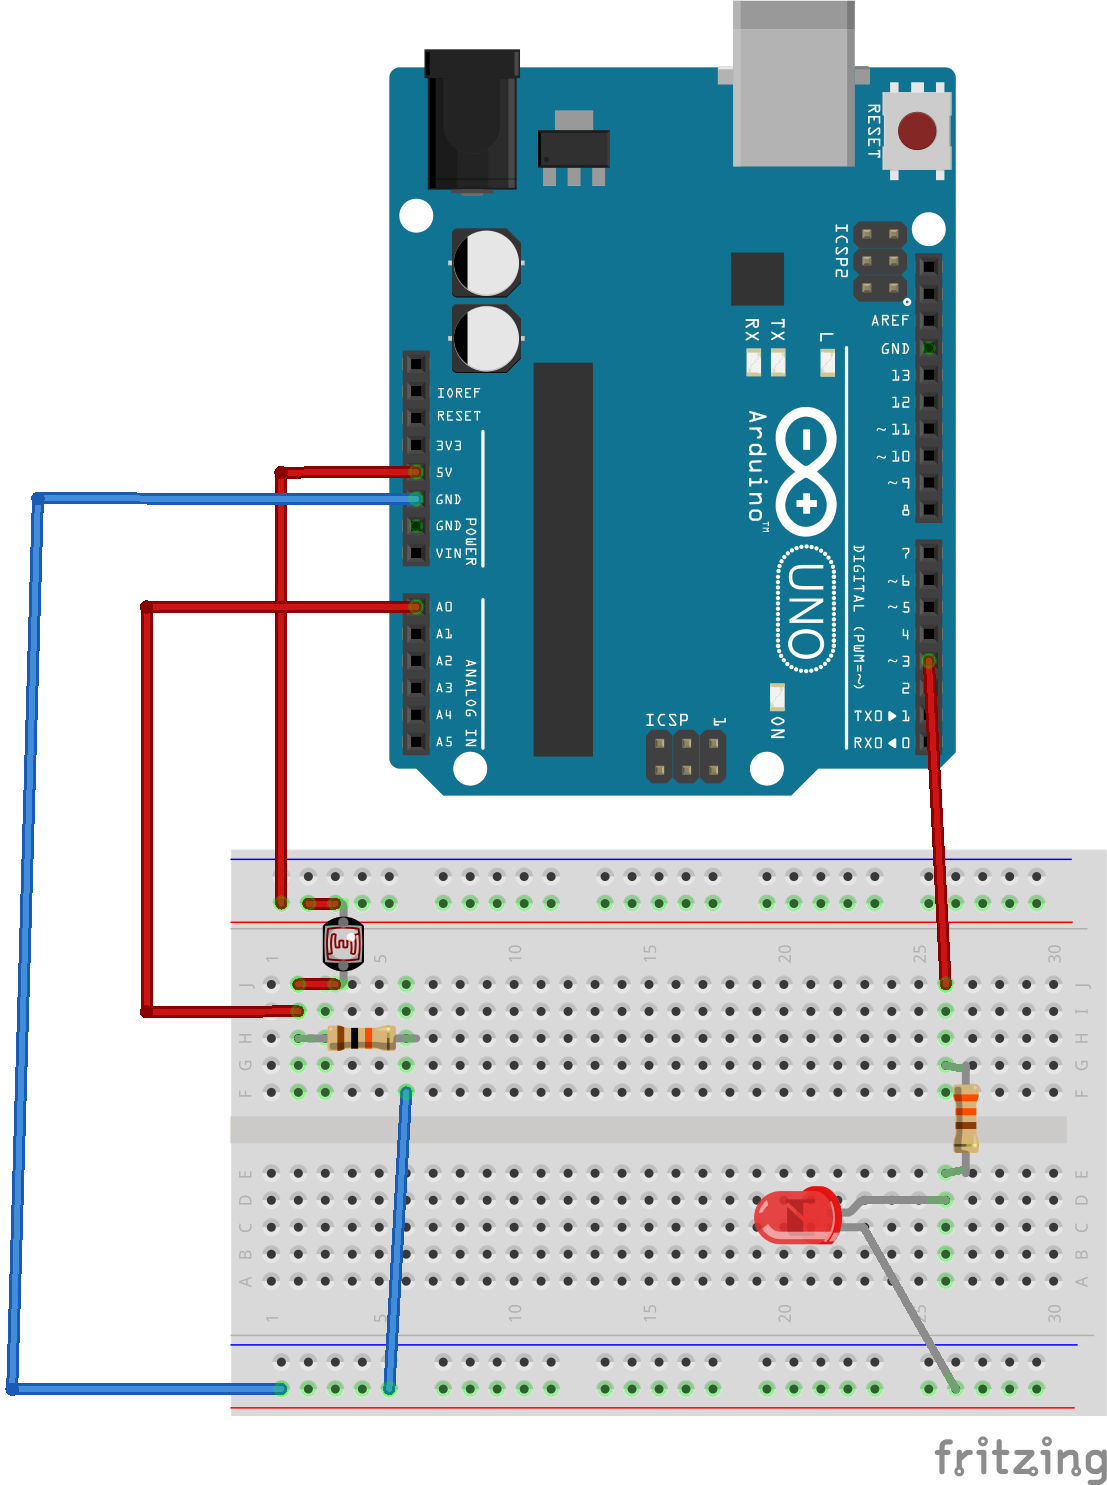
\includegraphics[width=7.0cm]{images/kadai2-3-2_bread.png}
\caption{発展課題2.3.2の配線図}
\label{fig:hattenkadai2-3-2bread}
\end{center}
\end{figure}

また,以下ソースコード\ref{code:hattenkadai2-3-2}にプログラムを示す.

\begin{lstlisting}[caption=発展課題2.3.2,label=code:hattenkadai2-3-2][H]
//値を定義
const int LED_PIN = 9;
void setup() {
  Serial.begin(9600);
  // シリアル通信を9600kbpsで初期化
  pinMode(LED_PIN,OUTPUT);
  //LEDを出力に設定
}
void loop() {
  int sensorValue = analogRead(A0);//A0ピンのAD変換結果を取得する.
  float vo = sensorValue*(5.0/1024.0);//デジタル値を電圧値に変換
  float L =222*vo;//電圧を照度値に変換
  Serial.println(L);//照度値をシステムモニタに表示
  analogWrite(LED_PIN,convert(L,0.0,2.17));//LED_PINポートにconvertの戻り値を出力
  delay(1);   //安定用
}

int convert(float lux,float lux_min,float lux_max){
  float out = lux/(lux_min - lux_max) *255;
  //照度値をPWMの出力に変換
  return out;//outを返す
}
\end{lstlisting}
プログラムで工夫した点は, convertの部分を関数化して使いやすくしたところである.

\section{発展課題2.3.3}

発展課題2.3.3で実装したブレッドボード配線図,プログラムおよび実験結果を報告せよ.2つのPWMの変化方法により,LEDの変化状態がどのように違ったか報告し,なぜ違いが生じているのか考察せよ.さらに,プログラムで工夫した点を記せ.

以下図\ref{fig:hattenkadai2-3-3bread}にブレッドボード配線図を示す.

\begin{figure}[H]
\begin{center}
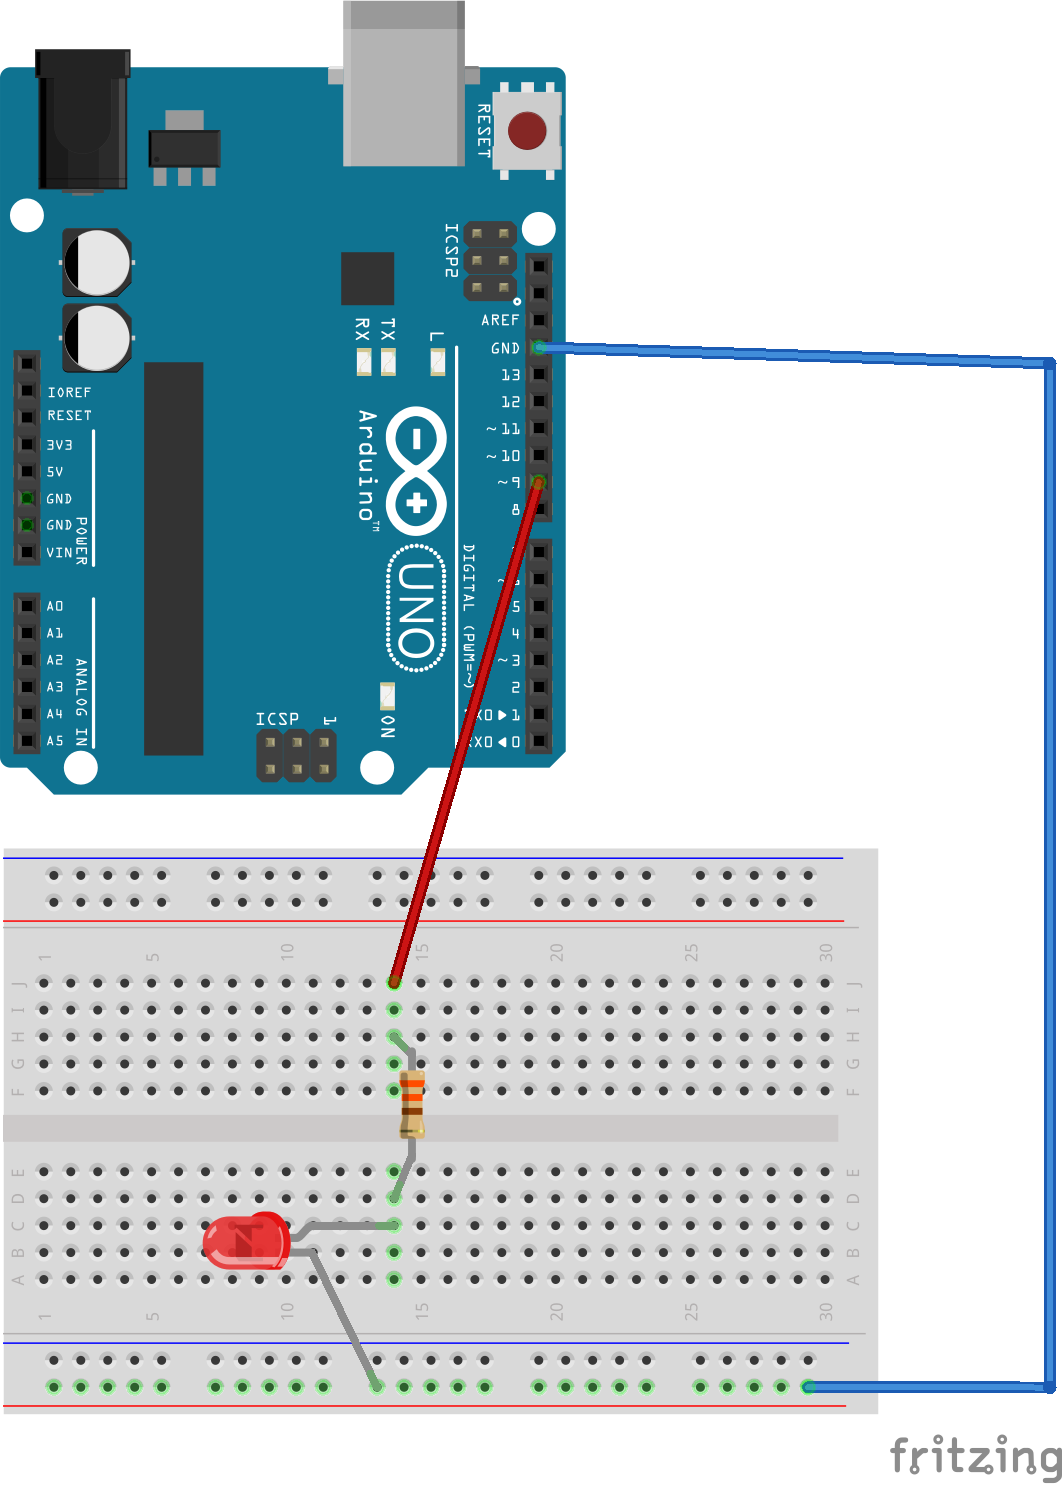
\includegraphics[width=7.0cm]{images/hatten2-3-3_bread.png}
\caption{発展課題2.3.3の配線図}
\label{fig:hattenkadai2-3-3bread}
\end{center}
\end{figure}

また,以下ソースコード\ref{code:hattenkadai2-3-3-nokogiri}にノコギリ波の,ソースコード\ref{code:hattenkadai2-3-3-sankaku}に三角波のプログラムを示す.

\begin{lstlisting}[caption=発展課題2.3.3ノコギリ波,label=code:hattenkadai2-3-3-nokogiri][H]
//値を定義
const int LED_PIN = 9;
void setup() {
  Serial.begin(9600);
  // シリアル通信を9600kbpsで初期化
  pinMode(LED_PIN,OUTPUT);
  //LED_PINを出力に設定 
}
void loop() {
  for(int i = 0; i < 256 ; i++){
    analogWrite(LED_PIN,i);//LED_PINにiを出力
    delay(1000/255);//255回で1秒待つ
  }
}
\end{lstlisting}

\begin{lstlisting}[caption=発展課題2.3.3三角波,label=code:hattenkadai2-3-3-sankaku][H]
//値を定義
const int LED_PIN = 9;
void setup() {
  Serial.begin(9600);
  // シリアル通信を9600kbpsで初期化
  pinMode(LED_PIN,OUTPUT);
  //LED_PINを出力に設定 
}
void loop() {
  for(int i = 0; i <=204 ; i++){//80パーセントは204
     analogWrite(LED_PIN,i);//iをLED_PINに出力
     delay(1000/204);//204回で1秒
  }
  for(int j = 204; j>0 ; j--){
    analogWrite(LED_PIN,j);//iをLED_PINに出力
    delay(1000/204);//204回で1秒待つ
  }
}
\end{lstlisting}
ノコギリ波では,LEDは徐々に明るくなったあと一定の明るさまで到達すると一気に明るさが落ち最初の状態となり,三角波では,LEDは徐々に明るくなったあと一定の明るさまで到達するとその後徐々に最初の明るさまで暗くなっていった.
これらの違いはPWMの変化方法が違うからである.ノコギリ波と三角波のグラフを見れば一目瞭然だが,ノコギリ派はある一定の値に達した後最初の値に戻るが,三角波はある一定の値に達した後は上昇した傾きと対照な傾きで値が下降していく.
プログラムで工夫した点は三角波の部分についてif文二つでわかりやすく簡潔にかいたことである.

\end{document}
